\chapter{ METHODOLOGY}

\noindent
In this chapter, we present the methodological framework adopted for our study. We detail the processes of data preparation, question-answer generation, model training, and evaluation, as well as the development of the visualization tool. Each section outlines the specific steps and techniques employed to ensure the reliability and reproducibility of our results.

\section{Dataset preparation}

\noindent
This section describes the procedures followed to curate and preprocess the datasets used in our research. We explain the selection of data sources, the integration of supplementary geographic and road network information, and the steps taken to ensure data quality and consistency prior to analysis.

\subsection{Data sources}

We leveraged the comprehensive China crime dataset published by \cite{Zhang2025CrimeDatasetChina}. To provide geographic context, we integrated administrative boundary data for China \citep{GeoJSON2025China} and road network data from OpenStreetMap \citep{Vargas2021OSM}. This enabled proximity calculations between criminal incidents and nearby roads, a significant variable within our analytical framework. Full dataset columns details are provided in Appendix \ref{appendix:dataset}.

\subsection{Data sources cleaning and normalization}

The dataset underwent thorough cleaning procedures, including handling of missing values, consolidating category columns through LLM-based classification, and standardization of date formats. All text fields were subsequently translated to English. To maintain analytical focus, we concentrated on the three provinces exhibiting the highest crime incidence during the 2017-2019 period: \textit{Jiangsu}, \textit{Guangdong}, and \textit{Zhejiang}.

\subsection{Question-Answer generation}

To develop our question-answer dataset, we first created 100 question templates (inspired by \citep{Dai2024QASTKG, Contractor2020QATourism}), covering different types of inquiries including spatio-temporal, comparative, and causal questions about crime data. These templates were designed to be adaptable for crime datasets from other countries as well.

We expanded this initial set through question augmentation techniques used by \cite{Yin2024MuMathCode, Li2024MuggleMath, Jain2024MetaFineTuning}, specifically rephrasing (with temperature setting of 0.5) and alteration (with temperature setting of 0.75) via few-shot prompting (see Table~\ref{tab:question_type_counts}, see prompt in Listings \ref{prompt:question_rephrasing} and \ref{prompt:question_augmentation}). These question categories are summarized in Table~\ref{tab:question_types}. Then, for each original question type, we selected random examples and developed Python code solutions manually. These hand-crafted solutions provided context for generating additional synthetic code answers using the DeepSeek V3 model with prompting (Listing~\ref{prompt:code_generation}) and nucleus-sampling \citep{Holtzman2020NucleusSampling, Ahmad2025OCRNVidia, Nvidia2024KaggleMath} (top\_p set to 0.95), generating new reasoning paths and coding approaches.


\begin{table}[H]
\centering
\begin{tabular}{lr}
\hline
\textbf{question\_type} & \textbf{\# count} \\
\hline
altered     & 3860 \\
paraphrased & 1732 \\
\hline
\end{tabular}
\caption{Distribution of question types in the dataset.}
\label{tab:question_type_counts}
\end{table}

\begin{table}[H]
\centering
\caption{Question types in the ChinaCrimeQACode dataset}
\label{tab:question_types}
\begin{tabular}{ll}
\toprule
\textbf{Question Type} & \textbf{Description} \\
\midrule
\texttt{spatial\_lookup} & Location-only questions \\
\texttt{temporal\_lookup} & Time-centric questions \\
\texttt{spatio\_temporal\_lookup} & Joint space-time filters \\
\texttt{comparative\_trends} & Rankings and evolution analysis \\
\texttt{causal\_contextual} & Event patterns and conditional queries \\
\texttt{hypotheticals\_counterfactuals} & Projections and counterfactual reasoning \\
\texttt{multi\_step\_aggregation} & Multi-step reasoning and aggregation \\
\bottomrule
\end{tabular}
\end{table}


\subsection{Dataset filtering}

To ensure quality, we verified that all LLM-generated Python solutions executed correctly. When errors occurred, we resubmitted queries to the LLM until either receiving a working solution or reaching the maximum retry limit. After that, we dropped the questions with no valid code solutions (limit exceeded, code with errors, or no code generated). Finally, we conducted manual reviews of all question-answer pairs to guarantee their quality.

\subsection{Dataset splitting}

The resulting dataset, which we named "ChinaCrimeQACode", contains around 5,000 question-code solution pairs, representing an adequate sample volume for effective model training \citep{Unsloth2024Dataset1}. We divided the dataset into training and test subsets using an 80/20 split to facilitate robust model training and comprehensive evaluation. The dataset is publicly available on HuggingFace for further research and development.  %  (Table~\ref{tab:dataset_split})
% This review process involved verifying that the answers were accurate, relevant, and aligned with the corresponding questions. We also ensured that the answers were concise and clear, making them suitable for use in our visualization tool.

% \begin{table}[H]
% \centering
% \begin{tabular}{lr}
% \hline
% \textbf{Split} & \textbf{Count} \\
% \hline
% train & 4513 \\
% test  & 1079 \\
% \hline
% \end{tabular}
% \caption{Dataset split distribution.}
% \label{tab:dataset_split}
% \end{table}


% TODO: poner ejemplo de question-answer pair

\section{Prompt Structuration}

All prompts were carefully designed to ensure the model understood the task requirements and could generate accurate code solutions. We describe below the structure of the prompts used both for answer generation and model training, highlighting how each layer of context helps to elicit precise and functional responses from the model. Full prompt examples are included in Appendix~\ref{appendix:prompts} for transparency and reproducibility.

\subsection{Answer generation prompt}

The answer generation prompt (Figure~\ref{fig:answer_generation_prompt_structure}) follows a layered structure designed to guide the DeepSeekV3 model through a rich, contextualized reasoning process. This prompt was used to create high-quality reference answers (i.e., ground truth) for training purposes.

At the top level, the \textbf{System Instructions} define the model’s role and restrict its scope of reasoning, ensuring consistency and relevance across generations. The \textbf{User Prompt} provides several critical components. First, the \textit{Dataset Context} introduces the \textit{Dataset Specification} of the three core dataframes: \texttt{crimes\_df}, \texttt{streets\_df}, and \texttt{geometries\_df}. This is followed by one-shot \textit{Reference Material}, offering prior examples (reference question and code) to scaffold the model’s behavior. Next, the prompt includes the target \textit{User Question}, which the model must answer, and a \textit{Detailed Task Description} outlining specific rules depending on whether the question is a rephrased or altered version of a known query.

Complementing this context, the \textbf{Dataset Specification} explicitly lists the column names, sample rows, data types, and semantic descriptions of each field. This encourages schema awareness and reduces ambiguity during code generation. Finally, an \textbf{Output Format} section prescribes the XML response schema to enforce structured and machine-readable outputs.

\begin{figure}[hbtp]
  \centering
  \includegraphics[width=0.65\textwidth]{images/answer_gen.png}
  \caption{Answer generation prompt structure}
  \label{fig:answer_generation_prompt_structure}
\end{figure}


\subsection{Training prompt structure}

For training, we employed a refined prompt format optimized for model fine-tuning and aligned with code generation best practices. The training prompt (Figure~\ref{fig:training_prompt_structure}) shares a similar foundational structure with the answer generation prompt but introduces stricter output constraints and excludes any example-based reasoning components.

At the top, the \textbf{System Instructions} define the model’s role as a geospatial crime analytics expert and enumerate the only allowed libraries. This early specification helps reduce hallucinations and ensures that generated solutions remain deterministic and reproducible.

The \textbf{Dataset Context} provides declarative metadata for the three key GeoDataFrames: \texttt{crimes\_df}, \texttt{streets\_df}, and \texttt{geometries\_df}, as well as their schema relations (e.g., spatial containment and joins). Unlike the answer generation prompt, the training prompt does \emph{not} include any one-shot reference material (i.e., no example question or sample code). This omission is intentional: it enforces that the model generalizes from the dataset schema and task formulation alone, without mimicking prior examples.

The \textbf{User Question} poses the target query in natural language. It is followed by a \textbf{Critical Requirements} block, which specifies strict constraints such as valid function signatures, use of allowed libraries, CRS alignment, and robust error handling.

The \textbf{Output Format} mandates that the response must be a single Python code block—excluding any natural language explanations or comments,thereby enabling seamless integration into downstream execution pipelines. Finally, the \textbf{Execution Directive} explicitly commands the model to begin coding immediately, ensuring a focused, code-only output from the first token.

\begin{figure}[hbtp]
  \centering
  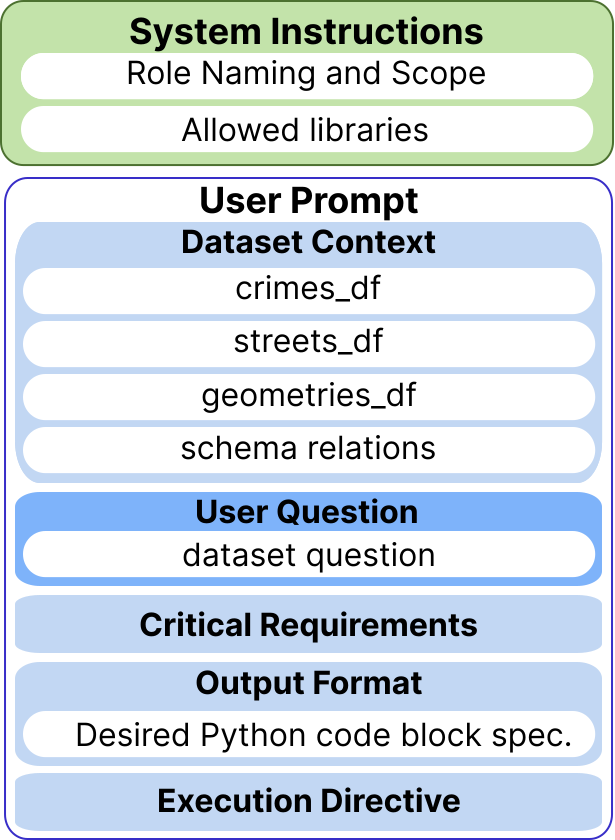
\includegraphics[width=0.3\textwidth]{images/prompt.png}
  \caption{Training prompt structure}
  \label{fig:training_prompt_structure}
\end{figure}


\section{Model Fine-Tuning}

We fine-tuned the Llama-3.1-8B Instruct model \citep{Grattafiori2024Llama3, Unsloth2024WhatModel} by implementing the techniques described in \cite{Pareja2024RecipesSFT}. For the fine-tuning process, we utilized Hugging Face Transformers alongside the Unsloth library to optimize computational resources and accelerate training, completing the entire procedure in approximately 3 hours using a single NVIDIA H100 GPU with 80GB memory provided by Lightning AI. This model was chosen as it represents a balance between size (8B), data science coding capabilities \citep{Lai2022DS1000}, and compatibility with Unsloth for fast and efficient fine-tuning.



\section{Model Evaluation}

% We adopted the approach proposed by \citep{Fleureau2024NuminaMath}, Self-Consistency Tool-Integrated Reasoning (SC-TIR) to evaluate our fine tuned model
For model evaluation, we adopted a comprehensive approach combining both automated and LLM-based assessment methods. Specifically, we used pass@k \citep{Levi2024SimpleModelInferenceScalingLaws} (with $k=16$ and multinomial sampling), where correctness was determined using an LLM-as-a-judge \citep{Li2025LLMJudge} (Appendix~\ref{appendix:prompts}) using GPT-4.1, and CodeBLEU \citep{Ren2020CodeBLEU}, which provides a purely quantitative measure of code generation quality. Additionally, we calculated the error percentage across all generated code samples to assess overall robustness. Finally, we performed Tool Integrated Reasoning (TIR) \citep{Fleureau2024NuminaMath} evaluations, allowing a single retry per question to mitigate frequent inference errors such as ZeroDivisionError and IndexError, while maintaining evaluation efficiency.

% TODO: poner que metodo de inferencia estamos usando, puede que sea greedy decoding

% The model was trained using QLoRA \citep{Dettmers2023QLoRA} with a rank of 64, alpha of 16, and a dropout rate of 0.05. 

% We employed a learning rate of 2e-4 with the AdamW optimizer and cosine learning rate scheduler with 100 warm-up steps. Training was performed for 3 epochs with a batch size of 16, using a maximum sequence length of 2048 tokens. To maintain training stability, we applied gradient clipping with a maximum norm of 1.0.

% For instruction tuning, we formatted our question-code pairs using a standard template that clearly specified the task context and expectations. Each question was prefaced with a system prompt indicating that the model should generate executable Python code to analyze crime data and answer the given question. 


\section{Inference Workflow}

This section describes the inference pipeline implemented for our case studies, detailing the process from user query to final response. As illustrated in Figure~\ref{fig:inference_pipeline}, the workflow consists of several key stages: first, the user query is processed by a fine-tuned Llama3-8B model, which generates multiple code solutions. Each code snippet is executed to produce corresponding outputs. Finally, a Llama3-8B-Base model performs summarization of these results to create the final response presented to the user.
%  This architecture enables robust and accurate responses to complex geospatial crime analytics queries.

\begin{figure}[H]
  \centering
  \includegraphics[width=0.9\textwidth]{images/inference_pipeline.drawio.png}
  \caption{Chat inference pipeline}
  \label{fig:inference_pipeline}
\end{figure}

% \section{Resume}

% This section provides a detailed overview of the methodology ...

% The section continues by detailing ...
